% Neutrino physics
% Target length: 30 pages

\graphicspath{{NeutrinoPhysics/Figs/}}

\chapter{Neutrino Physics}\label{chap:NeutrinoPhysics}

[Maybe should be a very very short chapter before then to `set the scene', mention the Standard Model and the general field of particle physics etc?]

Neutrino physics will be discussed! \\
\\
-- Background\\
-- Theory\\
-- Experiments\\
-- Future Experiments\\
\\
It may make sense to discuss the experiments as we go along...\\
\\
I think the chapter will work best with both past, present and future woven together.\\
And no distinct separation between theory and experiment (this is an experimental thesis after all...).\\
Can discuss the `neutrino problems' to motivate the theory of neutrino oscillations, and include the SNO and Kamiokande results within.\\
Then something similar with mass.\\
And as we get onto unanswered questions, can weave the propsed experiments into this.\\
I feel a section on the technology and concept of LAr TPCs will fit nicely into this setup.\\

%----------------------------------------------------------------------------------------------------------------------------------------------------------------------------
\section{Historical Context}\label{sec:HistoricalContext}

\subsection{Prediction of the Neutrino}\label{NeutrinoPrediction}

The neutrino was first posulated in 1930 by Wolfgang Pauli \cite{Pauli1930} in order to account for an inconsistency in the theory of $\beta$-decay.  In the apparent two-body decay
\begin{equation}
A \rightarrow B + e^-,
\end{equation}
kinematically the electron must be emitted with an energy given by
\begin{equation}\label{eq:BetaDecayEnergy}
E = \left( \frac{m_A^2 - m_B^2 + m_e^2}{2m_A} \right) c^2,
\end{equation}
where $m_{\alpha}$ is the mass of particle $\alpha$.  This energy is fixed given the masses of the particles; it was observed however that the electron energy followed a distribution (Figure \ref{fig:BetaDecayEnergy}), with Equation \ref{eq:BetaDecayEnergy} giving the maximum permitted energy.  The neutrino was postulated as a third final state particle in order to account for this result and retain energy conservation laws.  Pauli initially called the particle a \textit{neutron} (preempting the name Chadwick was to give his discovered particle in 1932) but his idea was met with much skeptism.  It was Fermi who named the new particle \textit{neutrino} (`little neutral one') when incorporating Pauli's hypoethesis into his theory of beta decay \cite{Fermi1934Italian,Fermi1934German,Wilson1968}.  With the huge success and acceptance of this theory, the field of neutrino physics was born.

\begin{figure}
  \centering
  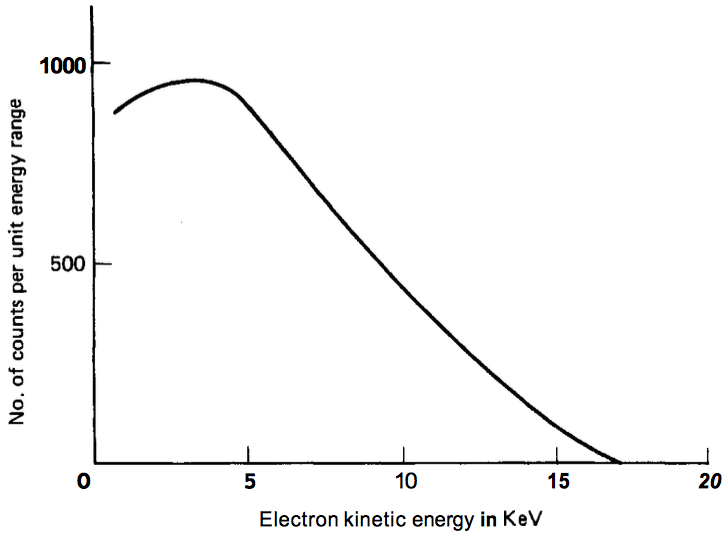
\includegraphics[width=10cm]{ElectronEnergySpectrumBetaDecay.png}
  \caption[Energy spectrum of the electron produced in beta decay.]{Energy spectrum of the electron produced in beta decay \cite{Lewis1970}.}
  \label{fig:BetaDecayEnergy}
\end{figure}

Further indications of the existence of the neutrino were provided by the studies of pion and muon decay by Cecil Powell's group at Bristol \cite{Lattes1947-159,Lattes1947-160}.  Topological investigatons of the newly discovered $\pi$ meson and its apparent decay into a lighter meson (now known to actually be the muon lepton) appear to hint at the presence of an additional, unknown, daughter particle \cite{Lattes1947-159}.  Given the constantly of the outcoming neutrino energy, it was that a two-body decay.  However, subsequent studies of the decay of this lighter `meson' implied a three-body decay involving two final state neutrinos, analogous to the implication of the neutrino by considering the electron energy distribution \cite{Brown1949}.

\subsection{Discovery of the Neutrino}\label{NeutrinoDiscovery}

The elegance of Fermi's theory convinced many physicists of the existence of the neutrino but until discovered experimentally it remained a hypothetical `book-keeping' device.  Given the elusive nature of neutrinos this wasn't for many years, leading to Pauli famously declaring ``I have done a terrible thing. I have postulated a particle that cannot be detected''.  However, a series of experiments conducted between 1953 and 1956 by Clyde Cowan and Frederick Reines confirmed the hypothesis and was later rewarded with the Nobel Prize in Physics in 1995.  Using the new technology of liquid scintillator detectors \cite{ReinesCowanLiquidScintillation}, they designed an experiment \cite{ReinesCowan1953Proposal} to study the (anti)neutrinos produced in inverse beta decay
\begin{equation}\label{eq:InverseBetaDecay}
  {\bar{\nu}}_e + p \rightarrow e^+ + n
\end{equation}
in the Hanford nuclear reactor in Washington, U.S.A.  Their signal comprised of an initial release of scintillation light when the positron annihilates with an electron, followed a characteristic time later by a gamma ray corresponding to the neutron capture.  The initial results from 1953 \cite{ReinesCowan1953} hinted at an excess over predicted background but the background proved to be much larger than anticipated, mainly due to an underestimation of the effects of cosmic rays.  A second experiment was conducted in 1956, this time 12~m underground and 11~m from the Savannah River reactor in South Carolina.  A neutrino detection rate of 2.9$\pm$0.2 per hour, greater than 20 times the accidental background rate was reported, confirming the previous indications \cite{ReinesCowan1956}.  The experimental discovery of the neutrino was confirmed.  [Bit more description? -- Describe detector, method for detecting positron.]

Ray Davis was also using nuclear reactors to study the interaction rates of neutrinos.  Using a detector of comprised of 3000 gallons of carbon tetrachloride (CCl$_4$) also close to the Savannah River reactor, Davis and Harmer searched for the interactions
\begin{equation}\label{eq:DavisAntineutrino}
  \bar{\nu} + \textnormal{Cl}^{37} \rightarrow \textnormal{Ar}^{37} + e^- \hspace{1.5cm} (\bar{\nu} + n \rightarrow p^+ + e^-);
\end{equation}
since it was known from Reines and Cowan that inverse beta decay
\begin{equation}\label{eq:DavisNeutrino}
  \nu + \textnormal{Cl}^{37} \rightarrow \textnormal{Ar}^{37} + e^- \hspace{1.5cm} (\nu + n \rightarrow p^+ + e^-)
\end{equation}
occurs, this facilites a comparison between the neutrino and the antineutrino.  They found the interaction shown in Equation \ref{eq:DavisAntineutrino} occurred at a rate less than 20 times that represented in Equation \ref{eq:DavisNeutrino}, implying for the first time a difference between neutrinos and antineutrinos \cite{Davis1959}.  This gave rise to the notion of `lepton number' and its conversation in physical interactions.

It was few years before the next chapter in the history of neutrinos, the discovery of the muon neutrino in 1962 at Brookhaven \cite{Danby1962}.  It was noted the apparently permitted decay
\begin{equation}
\mu^- \not\rightarrow e^- + \gamma
\end{equation}
is never observed, inciting the possibility of two distinct neutrinos.  In order to test this, Lederman, Schwarz and Steinberger used a muon neutrino beam to look for two separate interactions:
\begin{align}
  \bar{\nu}_{\mu} + p^+ &\rightarrow \mu^+ + n, \\
  \bar{\nu}_{\mu} + p^+ &\rightarrow e^+ + n.
\end{align}
With only one type of neutrino, each interaction would be expected to occur at around the same rate.  The beam was produced by accelerating protons up to 15 GeV and using a Beryllium target to create secondary mesons, decaying to produce neutrinos with energies up to 1 GeV.  34 muon tracks were detected (with an estimated background from cosmic muons of 5) and no events consistent with electrons were observed.  This remarkable result can only be rivalled by the technological advancements required; it was the first experiment to construct and use an artificial neutrino beam (common to all contemporary long-baseline experiments) and used 13.5~m thick steel from a dismantled battleship in order to ensure only neutrinos arrived at the spark chamber detector.  This discovery was rewarded with the Nobel Prize in 1988.

A third generation of lepton, the $\tau$, was discovered in 1975 by Martin Perl and his team at SLAC \cite{Perl1975}, completing the set of three charged leptons.  They reported 64 events of the form
\begin{equation}
  e^+ + e^- \rightarrow e^{\pm} + \mu^{\mp} + \ge 2 \textnormal{ undetected particles},
\end{equation}
using the energy and angle distributions to predict at least two additional particles.  They claimed `no conventional explaination' could account for these events and proposed the existence of a heavier charged lepton as an intermediate stage:
\begin{equation}
  e^+ + e^- \rightarrow \tau^+ + \tau^- \rightarrow e^{\pm} + \mu^{\mp} + 4\nu.
\end{equation}
The $\tau$ lepton was subsequently characterised by further experiments at by the Mark I detector at SLAC \cite{Feldman1977} and by the PLUTO collaboration at DESY \cite{Burmester1977}.  This result heavily implied the existence of an associated neutrino to complete the symmetry obvserved in the first two lepton couplets.

Further evidence for a third neutrino was provided by four experiments using the Large Electron-Positron Collider (LEP) at CERN in 1989 which were studying the production of the newly discovered Z$^0$ boson \cite{DeCamp1989,Adeva1989,Akrawy1989,Aarnio1989}.  The width $\Gamma_Z$ of the Z$^0$ resonance is dependent on the partial widths relating to final state charged leptons, hadrons and neutrinos;
\begin{equation}
  \Gamma_Z = N_{\nu} \Gamma_{\nu} + 3 \Gamma_{ee} + \Gamma_{\mathrm{hadron}},
\end{equation}
where $N_{\nu}$ is the number of light ($m_{\nu} \le \frac{m_Z}{2}$) active neutrinos.  Figure \ref{fig:LEPZ0Resonance} shows this resonance for a range of $N_{\nu}$ hypotheses; fitting to the data yields a value of $2.984 \pm 0.008$ neutrino flavours \cite{Schael2006}.

\begin{figure}
  \centering
  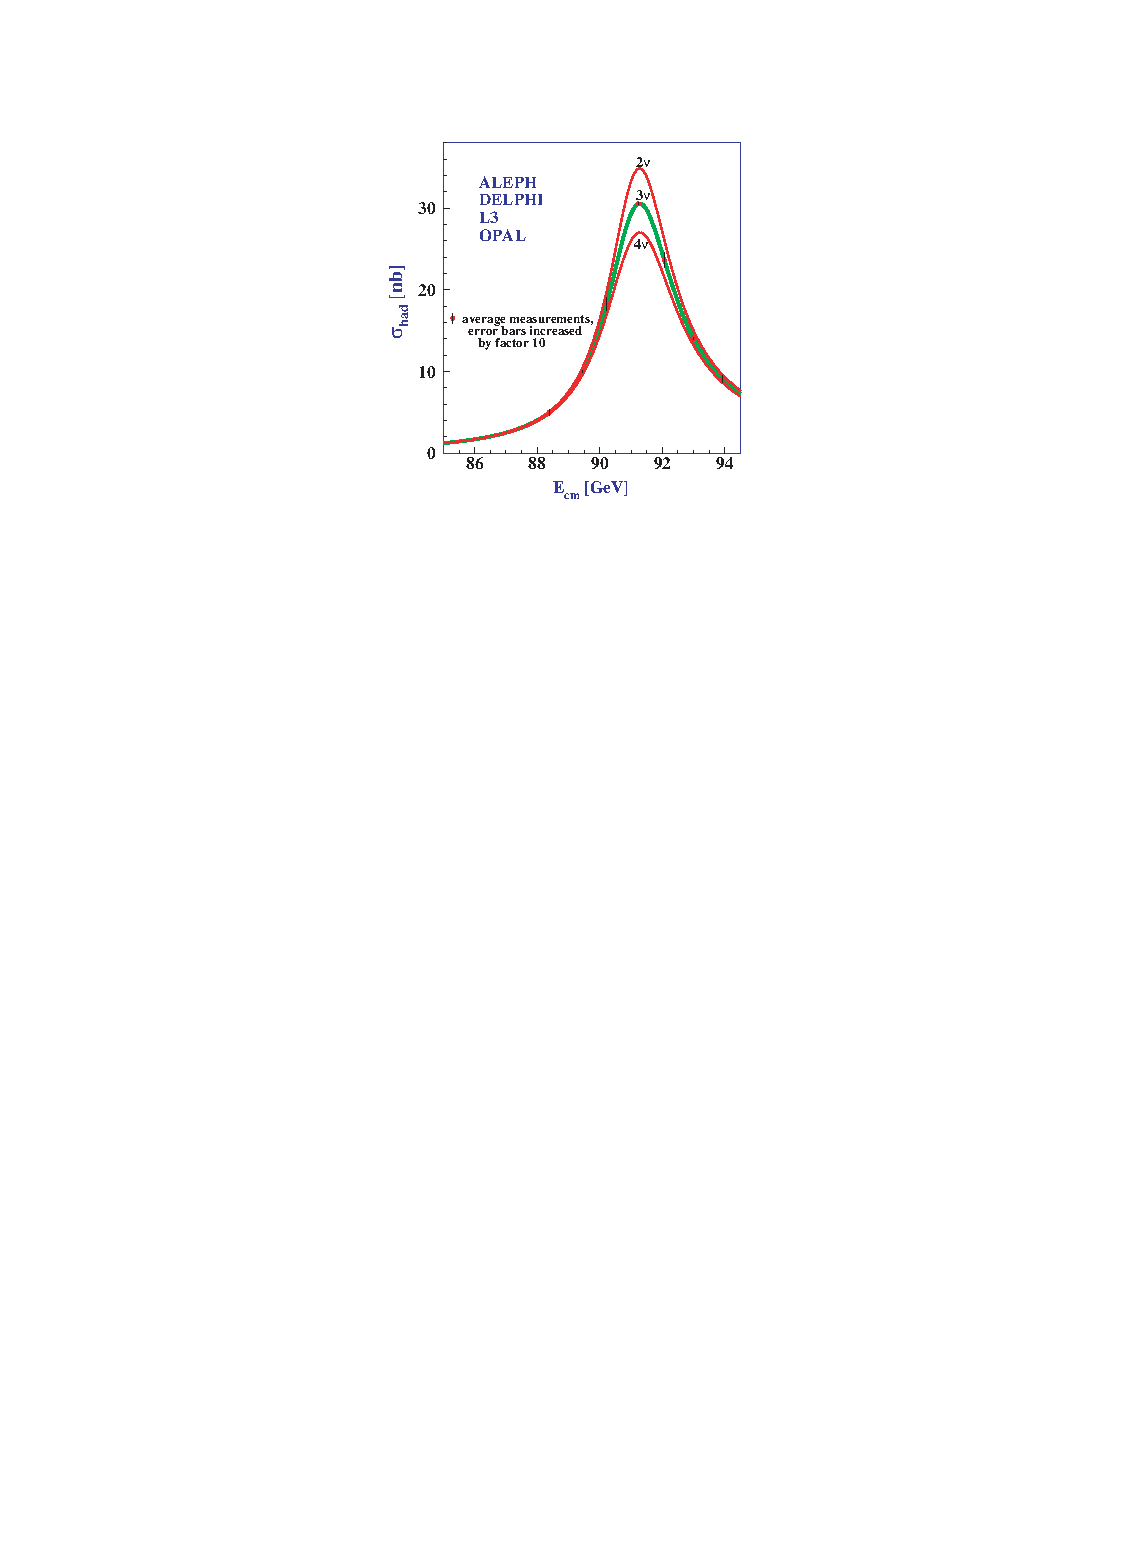
\includegraphics[width=12cm]{LEPZ0Resonance.pdf}
  \caption[Measurements of the hadron production cross-section around the Z resonance.]{Measurements of the hadron production cross-section around the Z resonance.  The curves indicate the predicted cross-section for two, three and four neutrino species with SM couplings and negligible mass.  Taken from \cite{Schael2006}.}
  \label{fig:LEPZ0Resonance}
\end{figure}

The extremely precise measurement reported by the LEP experiments was enough for a lot of physicists to claim indisputable evidence for the existence of the tau neutrino; it was partly for this reason that its experimental discovery wasn't until 25 years after the addition of the $\tau$ lepton to the Standard Model.  However, in 2000 the DONUT experiment at Fermilab, IL, U.S.A. finally reported direct detection of the tau neutrino \cite{Kodama2001}.  DONUT (Direct Observation of NuTau), as the name suggests, was designed specifically for the purpose of finding the third neutrino.  It did this by identifying the $\tau$ as the only lepton at the interaction vertex from a $\nu_{\tau}$ beam created by firing 800 GeV protons from the Tevatron at a tungsten beam dump.  The mean energy of the $\nu_{\tau}$s detected at the emulsion target 36~m downstream was 111~GeV, produced by the decay of a $D_S$ meson to a $\tau$ lepton and a $\bar{\nu}_{\tau}$ neutrino followed by the decay of the $\tau$ to a $\nu_{\tau}$.  Four events were found, above a predicted background of $0.34\pm0.05$, consistent with the Standard Model description of the tau neutrino.

\subsection{The Solar Neutrino Problem}\label{SolarNeutrinoProblem}

It has been known since the 1930s, when Hans Bethe started developing the ideas of stellar nucleosynthesis \cite{Bethe1939}, that an adundance of electron neutrinos is created as byproducts of the nuclear processes powering the Sun.  The Standard Solar Model (SSM), established by John Bahcall in 1968 \cite{Bahcall1968}, explains the nuclear fusion processes responsible for powering stars.  For stars the size of the Sun, this is dominated by the \textit{proton-proton chain}; heavier stars follow the \textit{CNO cycle}.  Figure \ref{fig:SolarNeutrinos} shows the energy spectra of neutrino released during reactions occuring during both chains.

\begin{figure}
\centering
  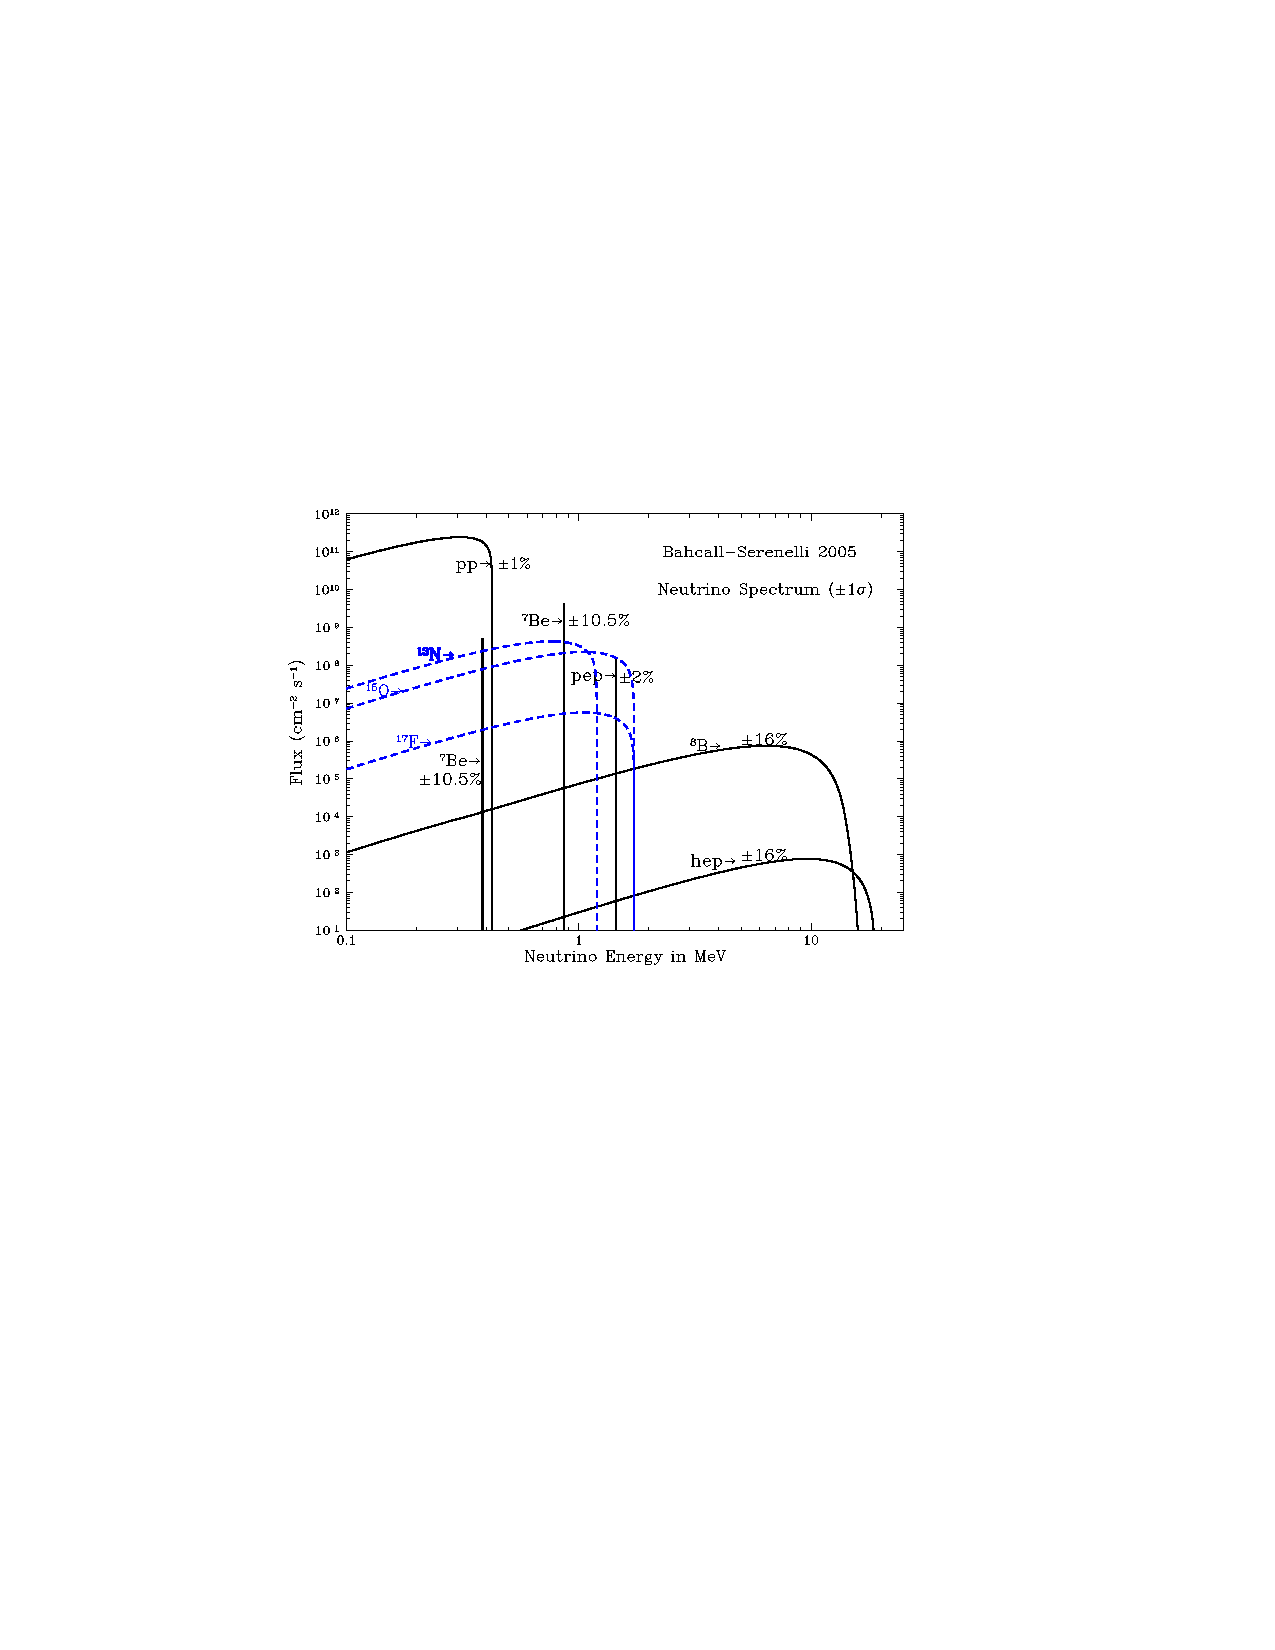
\includegraphics[width=12cm]{SolarNeutrinos.pdf}
  \caption{Solar neutrino energy spectra as predicted by the Standard Solar Model \cite{Bahcall2005}.  The solid lines repesent neutrinos produced during the p-p chain and dashed line represent neutrinos from the CNO cycle.  Each spectrum illustrates a particular reaction during the process of a given chain.}
  \label{fig:SolarNeutrinos}
\end{figure}

Ray Davis, in collaboration with Bahcall, conducted the first experiment to detect these solar neutrinos in 1968.  Using a similar detection technique to his previous experiments, Davis used a 380~m$^3$ tank of tetrachloroethene (C$_2$Cl$_4$) to detect neutrinos via the inverse beta decay reaction detailed in Equation \ref{eq:DavisNeutrino}.  Given the threshold for this reaction is 0.814 MeV, the main sources of neutrinos probed by this experiment were Be$^7$ and B$^8$.  In order to eliminate backgrounds from cosmic rays, Davis constructed his experiment 4850~ft underground at the Homestake mine near Lead, SK, U.S.A.  It is worth noting, in a pleasing neutrino-full-circle, this is exactly where the far detector for the DUNE experiment will be housed.  The Davis Homestake experiment ran for 25 years but the results obtained \cite{Cleveland1995} disagreed quite strongly with the SSM \cite{Bahcall1995}, consistently measuring solar electron neutrinos at a rate around a third that predicted by the model.  This became known as the `solar neutrino problem', and Davis was awarded the Nobel Prize for his work on this famous experiment in 2002.

The subsequent radiochemical experiments SAGE (from 1990) and GALLEX (from 1991) were sensitive to the large flux of \textit{pp} neutrinos by utilising a Ga$^{71}$ target and the lower threshold reaction
\begin{equation}
\nu + \textnormal{Ga}^{71} \rightarrow \textnormal{Ge}^{71} + e^-.
\end{equation}
These experiments also reported `missing' neutrinos, determining capture rates of $66.6^{+6.8+3.8}_{-7.1-4.0}$~SNU (SAGE) \cite{Abdurashitov1994} and $77.5\pm6.2^{+4.3}_{-4.7}$~SNU (GALLEX) \cite{Anselmann1992}, disagreeing with the SSM prediction of 130~SNU \cite{Hampel1999}.  There appeared to be a problem -- either the SSM was incomplete and incorrectly overpredicted the amount of electron neutrinos or hints of new physics were beginning to appear in the experiment data.

\subsection{The Atmospheric Neutrino Anomaly}\label{sec:AtmosphericNeutrinoAnomaly}

Another abundent source of natural neutrinos come from cosmic rays interacting with the upper atmosphere and producing `atmospheric neutrinos', typically via the interactions \cite{Gaisser1990}
\begin{align}
  \pi^+ \rightarrow \mu^+ + \nu_{\mu}, &\hspace{1.5cm} \mu^- \rightarrow e^- + \bar{\nu}_e + \nu_{\mu} \\
  \pi^- \rightarrow \mu^- + \bar{\nu}_{\mu}, &\hspace{1.5cm} \mu^+ \rightarrow e^+ + \nu_e + \bar{\nu}_{\mu}.
\end{align}
Since the decay lengths and kinematics are well known, the predicted ratio of muon to electron neutrinos can be calculated to a good accuracy.  This ratio can be compared to an experimentally determined ratio and analysed as a measure of the efficiacy of the model.

It was first noticed as early as the late 1970s by experiments designed to search for nucleon decay predicted by the then-popular Grand Unified Theories that the measured flux did not correspond to that predicted by the theory.  The IMB \cite{Haines1986} and Kamioka \cite{Hirata1988} experiments both noticed deficiencies in the ratio between muon and electron neutrinos compared to that prediced by the models.  These experiments utilised large tanks of pure water surrounded by Photo-Multiplier Tubes (PMTs) to detect neutrinos via the Cherenkov radiation created by their charged leptonic daughter particles.  Using ring-imaging techniques, it is possible to distinuish between electron-like and muon-like events and therefore identify the flavour of the incoming neutrino.  The problem implied by these measurements is known as the `atmospheric neutrino anomaly'.

Various other experiments over the following twenty years also reported similar measurements, suggesting an excess of electron neutrinos over prediction, a deficit in the number of muon neutrinos, or both.  Results from numerous experiments are shown in Figure \ref{fig:AtmosphericNeutrinoAnomaly}.  Most experiments report a discrepency, with its size seemingly dependent on the energy region being studied.  The experiments reporting a ratio consistent with one were much smaller than the others, and with more statistics they also started observing similar effects.  This anomaly, along with the issue of the solar neutrino problem, strongly hinted at a problem with our understanding of neutrino physics.

\begin{figure}
  \centering
  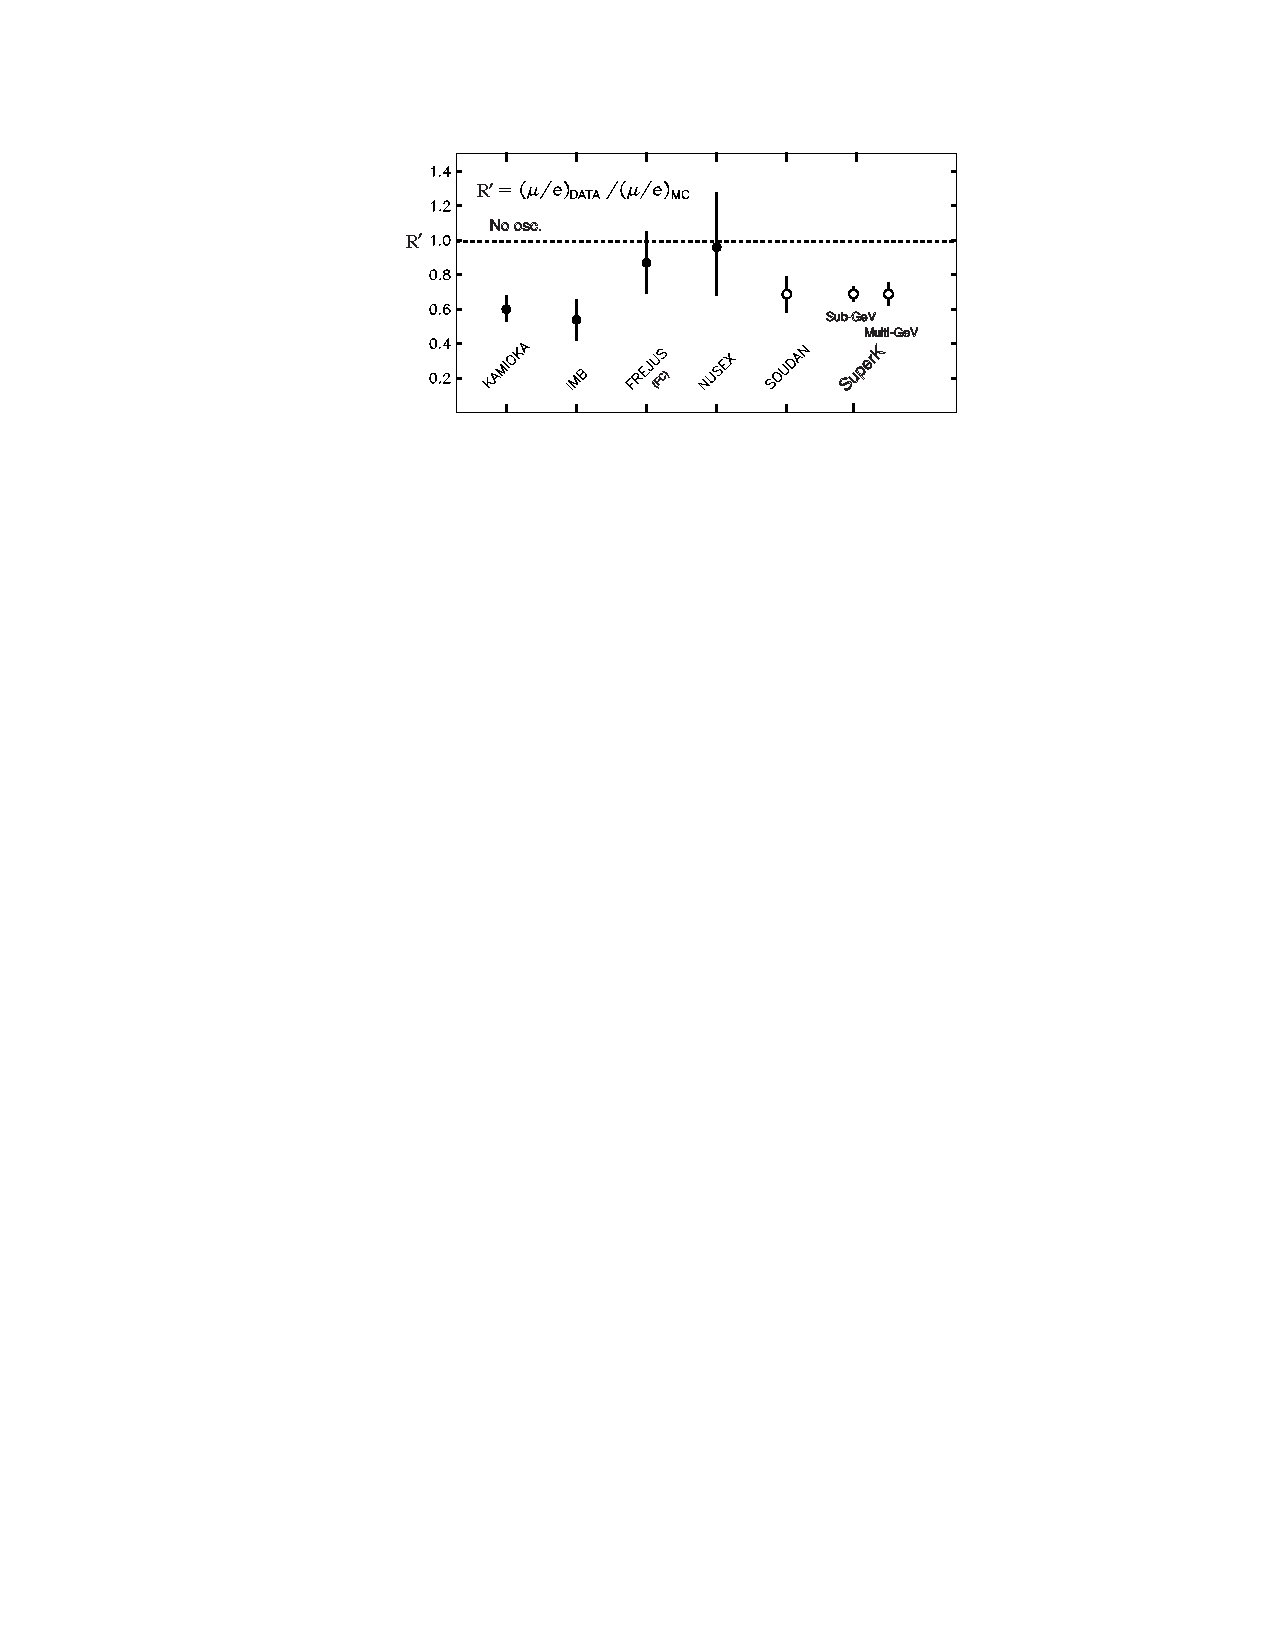
\includegraphics[width=12cm]{AtmosphericNeutrinoAnomaly.pdf}
  \caption{The double ratio \textit{R} of muon to electron neutrino events showing data divided by expectation \cite{Mann1999}.  Various underground atmospheric neutrino detectors are shown.}
  \label{fig:AtmosphericNeutrinoAnomaly}
\end{figure}

\subsection{The Evidence for Neutrino Oscillations}\label{sec:EvidenceNeutrinoOscillations}

The concept of neutrino oscillations is the idea that a neutrino created in a certain flavour state may not necessary be detected in the same flavour state after it has propgated over some distance and time.  It was first postulated as an explaination of the solar neutrino problem by Pontecorvo in 1968 \cite{Pontecorvo1968}, having initially proposed the phonomenon in 1957 as an analogy to $\textnormal{K}^0 \rightarrow \widetilde{\textnormal{K}}^0$ transition in the quark sector \cite{Pontecorvo1957}.  It offers an elegant solution to both the solar neutrino problem and the atmospheric neutrino anomaly by explaining where the `missing' neutrinos had gone; it is possible they had simply `oscillated' to a different flavour and therefore would not be detected as expected.  Whilst there was speculation that neutrino oscillations may be the explanation behind the issues observed in the data much sooner \cite{Casper1991,BeckerSzendy1992}, definite proof was not provided until the late 1990s.  The Kamiokande experiment in Japan (an upgrade from the Kamioka experiment noted previously) and the SNO experiment in Sudbury, Canada produced results showing indisputible evidence for neutrino oscillations and providing explanations for all previous discrepencies observed.  This result was monumental and the work of both collaborations was rewarded in 2015 when the Nobel Prize was awarded to T. Kajita and A. McDonald, from Kamiokande and SNO respectively.  The story of neutrino physics can be considered a triumph for the scientic method.

Kamiokande and SNO!

%----------------------------------------------------------------------------------------------------------------------------------------------------------------------------
\section{Neutrino Oscillations}\label{sec:NeutrinoOscillations}

The theory of neutrino oscillations is basically the quantum mechanics of mixed states and was developed on top of Pontecorvo's work by Ziro Maki, Masami Nakagawa and Shoichi Sakata \cite{MNS1962}.  If the neutrino flavour states can spontaneously convert from one to another, none can be considered as eigenfunctions of the Hamiltonian.  The true stationary states are the \textit{mass eigenstates} ($\nu_1$, $\nu_2$, $\nu_3$), of which the flavour states ($\nu_e$, $\nu_{\mu}$, $\nu_{\tau}$) can be considered linear superpositions:
\begin{equation}
  \begin{pmatrix}
    \nu_e \\
    \nu_{\mu} \\
    \nu_{\tau} \\
  \end{pmatrix}
  =
  U^*_{\textnormal{PMNS}}
  \begin{pmatrix}
    \nu_1 \\
    \nu_2 \\
    \nu_3 \\
  \end{pmatrix},
  \label{eq:FlavourMassStates}
\end{equation}
where $U_{\textnormal{PMNS}}$ is the PMNS mixing matrix which described the flavour composition of each of the mass eigenstates, and vice versa.  If the PMNS matrix were diagonal, each flavour state would correspond to a single mass state and oscillations would not occur.

Just as the flavour states are a superposition of mass states
\begin{equation}\label{eq:FlavourSuperposition}
  \ket{\nu_{\alpha}} = \sum_i U^*_{\alpha i} \ket{\nu_i},
\end{equation}
the mass states can also be considered a superposition of flavour states
\begin{equation}\label{eq:MassSuperposition}
  \ket{\nu_i} = \sum_{\alpha} U_{\alpha i} \ket{\nu_{\alpha}}.
\end{equation}

For the three neutrino case, the PMNS matrix, decomposed into its three axial rotations, can be expressed as
\begin{equation}
  U_{\alpha i} \equiv
  \underbrace{
    \begin{pmatrix}
      1 & 0 & 0 \\
      0 & c_{23} & s_{23} \\
      0 & -s_{23} & c_{23} \\
    \end{pmatrix}
  }_{\textnormal{`Atmospheric' term}}
  \underbrace{
    \begin{pmatrix}
      c_{13} & 0 & e^{-i\delta} s_{13} \\
      0 & 1 & 0 \\
      -e^{-i\delta} s_{13} & 0 & c_{13} \\
    \end{pmatrix}
  }_{\textnormal{`Accelerator' or `Reactor' term}}
  \underbrace{
    \begin{pmatrix}
      c_{12} & s_{12} & 0 \\
      -s_{12} & c_{12} & 0 \\
      0 & 0 & 1 \\
    \end{pmatrix}
  }_{\textnormal{`Solar' term}}
  ,
  \label{eq:PMNS}
\end{equation}
where $c_{ij} \equiv \cos{(ij)}$, $s_{ij} \equiv \sin{(ij)}$ and $\delta$ is a CP-violating phase factor.  Each axial component is often referred to by the means with which they are studied, as shown in Equation \ref{eq:PMNS}.

The weak interaction couples to the flavour eigenstates so neutrinos are always created and detected as flavour states.  However, they propagate as mass states since it is these which are eigenstates of the Hamiltonian.  Due to the misalignment of the flavour and mass states, oscillations can be shown to occur.  A neutrino created with flavour $\alpha$ is a superposition of all the mass states (Equation \ref{eq:FlavourSuperposition}).  These states progagate as a plane wave, evolving in time and space such that
\begin{equation}\label{eq:MassTimeEvolution}
  \ket{\nu_i(x,t)} = \ket{\nu_i (0)} e^{-i \textbf{x} \cdot \textbf{p}},
\end{equation}
where \textbf{x} and \textbf{p} are the 4-position and 4-momentum of the neutrino respectively.  From Equations \ref{eq:FlavourSuperposition} and \ref{eq:MassTimeEvolution}, the evolution of the flavour states over space and time is therefore
\begin{align}
  \nonumber \ket{\nu_{\alpha}(x,t)} &= \sum_i U_{\alpha i}^* \ket{\nu_i (x,t)} \\
  \label{eq:FlavourTimeEvolution} &= \sum_i U_{\alpha i}^* e^{-i \textbf{x} \cdot \textbf{p}} \ket{\nu_i(0)} .
\end{align}
In the ultra-relativistic limit, the mass of the neutrino is negligble compared to its momentum ($m_i \ll \vec{p}$) and $\vec{x} \approx ct$;
\begin{align}
  \label{eq:RelativisticEnergy} E_i &= \sqrt{|\vec{p}|^2+m_i^2} = \vec{p}\sqrt{1+\frac{m_i^2}{|\vec{p}|^2}} \approx \vec{p}+\frac{m_i^2}{2\vec{p}} \\
  \label{eq:RelativisticEnergyMomentum} \textbf{x}\cdot\textbf{p} &= E_i t - \vec{x}\cdot\vec{p} = \vec{p}\cdot t + \frac{m_i^2}{2\vec{p}}t - \vec{x}\cdot\vec{p} \approx \frac{m_i^2}{2\vec{p}}\vec{x} = \frac{m_i^2}{2p}x ,
\end{align}
assuming the neutrino displacement is in the direction of its momentum and using natural units ($c \equiv \hbar \equiv 1$).  Thus, using Equations \ref{eq:FlavourTimeEvolution}, \ref{eq:RelativisticEnergyMomentum} and \ref{eq:MassSuperposition},
\begin{align}
  \nonumber \ket{\nu_{\alpha}(x,t)} &= \sum_i U_{\alpha i}^* e^{-i \frac{m_i^2}{2p} x} \ket{\nu_i (0)} \\
  \label{eq:FlavourEvolution} &= \sum_i \sum_{\beta} U_{\alpha i}^* e^{-i \frac{m_i^2}{2p} x} U_{\beta i} \ket{\nu_{\beta}}.
\end{align}

The probability of a neutrino created in flavour state $\alpha$ being observed in flavour $\beta$ can be determined from Equation \ref{eq:FlavourEvolution}
\begin{align}
  P(\alpha \rightarrow \beta) &= |\braket{\nu_{\alpha}}{\nu_{\beta}(x,t)}|^2 \\
  &= \left[ \sum_i U_{\alpha i} e^{i \frac{m_i^2}{2p} x} U_{\beta i}^* \right] \left[ \sum_j U_{\alpha j}^* e^{-i \frac{m_j^2}{2p} x} U_{\beta j} \right] \\
  &= \sum_{i,j} U_{\alpha i} U_{\alpha j}^* U_{\beta j} U_{\beta i}^* e^{i \frac{m_i^2-m_j^2}{2p} x},
\end{align}
and is observed to be dependent on the neutrino momentum, the difference between the squared masses of the flavour states, the propagation distance and the relative mixing of the two flavour states encoded in the matrix elements $U$.

An accelerator based neutrino experiment, such as DUNE, will typically use a $\nu_{\mu}$-dominated beam and look for \textit{muon neutrino disappearance} ($P(\nu_{\mu}\rightarrow \nu_{\mu})$) and \textit{electron neutrino appearance} ($P(\nu_{\mu}\rightarrow \nu_e)$).  In this case, also in the relavistic limit, the relevant appearance and disappearance probabilities can be approximated, respectively, as
\begin{align}
  \label{eq:ElectronNeutrinoAppearance} P(\nu_{\mu} \rightarrow \nu_e) &\approx \sin^2{2\theta_{13}} \sin^2{\theta_{23}} \sin^2 {\left( 1.27 \frac{\Delta m_{13}^2 L}{E} \right)} \\
  \label{eq:MuonNeutrinoDisappearance} P(\nu_{\mu} \rightarrow \nu_{\mu}) &\approx 1 - \cos^4{\theta_{13}} \sin^2{2\theta_{23}} \sin^2{ \left( 1.27 \frac{\Delta m_{23}^2 L}{E} \right) },
\end{align}
where $\Delta m_{ij}^2 \equiv m_i^2-m_j^2$ is the \textit{mass squared splitting} in eV, $L$ is the distance propagated in km and $E$ is the neutrino energy in GeV.

\subsection{Matter Effects}\label{sec:MatterEffects}

The oscillations considered thus far are \textit{vacuum oscillations} which occur due to the mixing of the neutrino mass and flavour states.  When neutrinos propagate through matter, an additional potential can be shown to also produce oscillations, which would occur even in the case of no vacuum oscillations.

As neutrinos pass through matter, coherent scattering (scattering in which the neutrino state is unchanged) due to neutrino interactions with matter cause neutrinos to feel a potential.  As normal matter is composed of electrons, rather than their heavier counterparts muons and taus, electron neutrinos are affected more by this potential.  The mechanism for this is demonstated in Figure \ref{fig:MatterEffects}.  This gives rise to an additional effective mass splitting between the electron neutrino and the other flavours and therefore results in the possibility of oscillations \cite{Wolfenstein1978}.

\begin{figure}
  \centering
  \begin{subfigure}{0.48\linewidth}
    \centering
    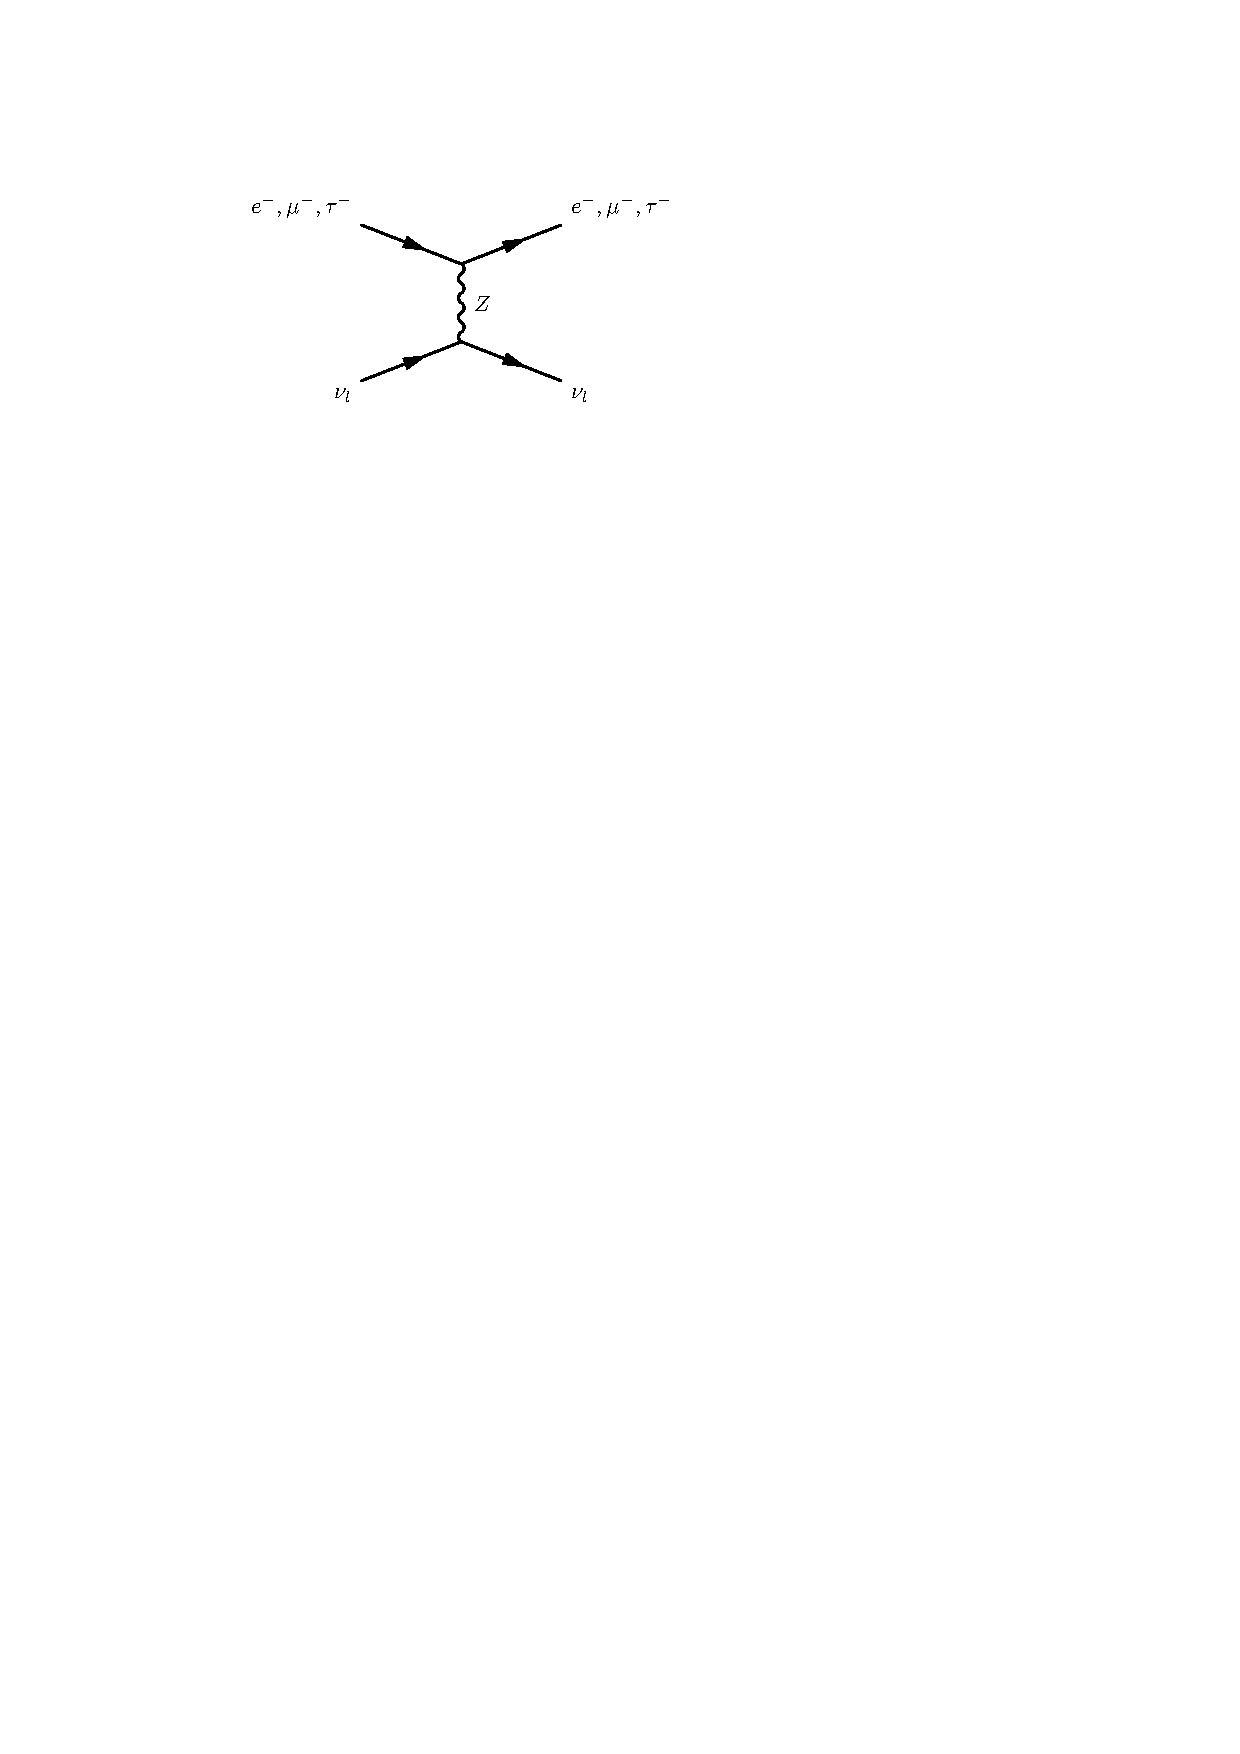
\includegraphics{MatterEffectsNC.pdf}
    \caption{Neutral current scattering.}
    \label{fig:MatterEffectsNC}
  \end{subfigure}
  \hfill
  \begin{subfigure}{0.48\linewidth}
    \centering
    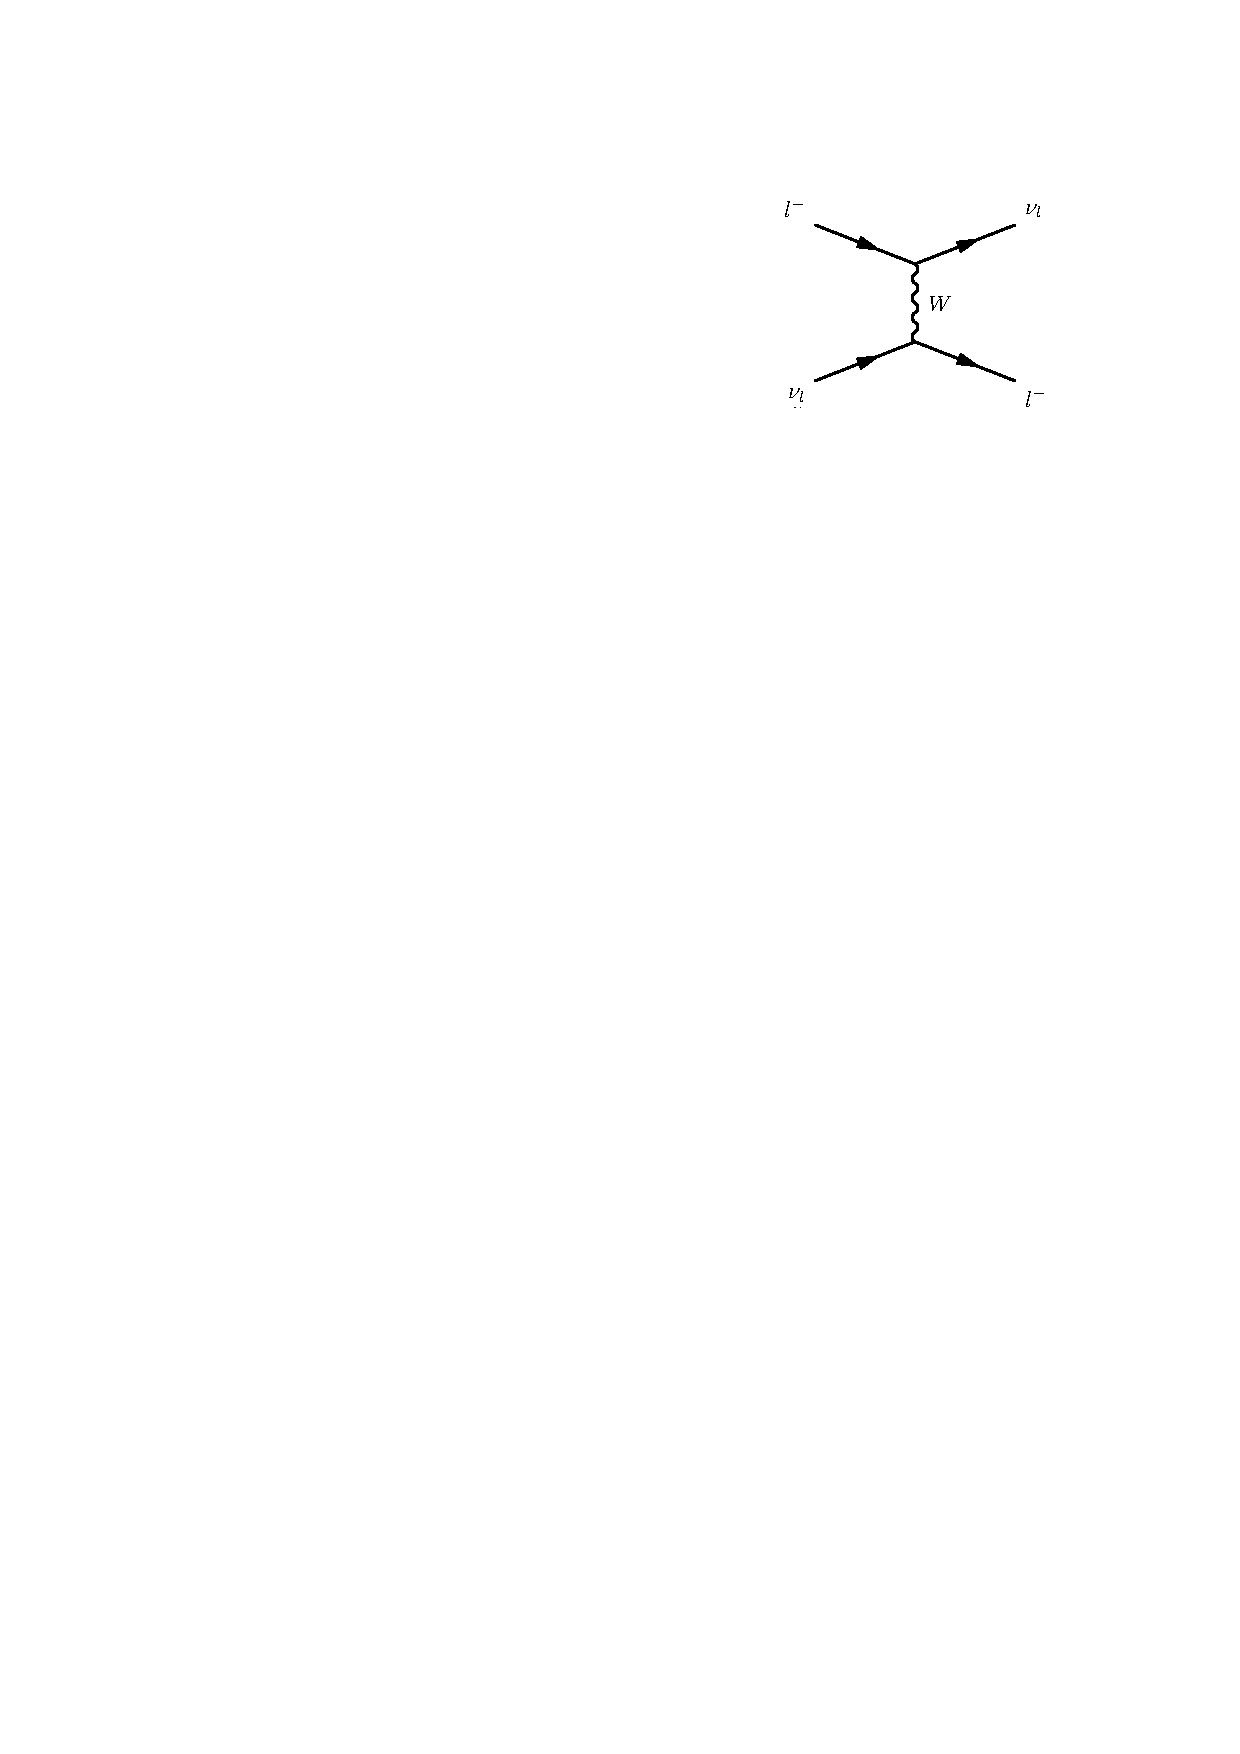
\includegraphics{MatterEffectsCC.pdf}
    \caption{Charged current scattering.}
    \label{fig:MatterEffectsCC}
  \end{subfigure}
  \caption{General scattering mechanics which occur as neutrinos pass through matter.  Neutral current scattering (Figure \ref{fig:MatterEffectsNC}) occurs for all neutrino flavour combinations whereas charged current scattering (Figure \ref{fig:MatterEffectsCC}) only occurs when the incoming leptons have the same flavour.}
  \label{fig:MatterEffects}
\end{figure}

\subsection{CP-Violation}\label{sec:CPViolation}

\subsection{Neutrino Mass}\label{sec:NeutrinoMass}

%----------------------------------------------------------------------------------------------------------------------------------------------------------------------------
\section{Current Understanding of Neutrino Physics}\label{sec:CurrentUndertstanding}

Including oscialliation parameters\\
Mass splittings and degeneracy\\
SN?\\

%----------------------------------------------------------------------------------------------------------------------------------------------------------------------------
\section{Future Neutrino Experiments}\label{sec:FutureNeutrinoExperiments}

%----------------------------------------------------------------------------------------------------------------------------------------------------------------------------
\section{The LAr TPC Concept [Lee -- could be in DUNE chapter?]}\label{sec:LArTPC}

The use of a liquid argon time projection chamber (LArTPC) as a high-precision fine-grained detector medium holds much promise for the successful resolution of the open questions in neutrino physics.  A great amount of R\&D work has taken place to advance the maturity of the technology and pioneering experiments, such as ICARUS \cite{ICARUS2004}, have further increased the understanding of the neutrino community of the detector techniques.  Past and currently running experiments at Fermilab, such as ArgoNeuT [], LArIAT [] and MicroBooNE [], are successfully using LArTPCs to take and analyse data and it seems certain to be the future of neutrino physics in the U.S.

This section will provide a brief history of LArTPC technology and motivate its potential when used in a huge experiment such as DUNE.  The basic operation of such a detector will also be described to provide background for discussion of the DUNE and 35t experiments, and of reconstruction in LArTPCs, in future chapters.

\subsection{A Brief History of Time (Projection Chambers)}\label{sec:LArTPCHistory}

The use of a time projection chamber as a potential particle detector was put forward by David Nygren in 1974 \cite{Nygren1974}.  He envisioned bubble-chamber quality data but with the possiblity of digital readout of the data, fascilitating extremely fine spatial resolution, good timing resolution and fast recovery after triggering.  The basic concept is a drift chamber containing a noble gas placed within a field to drift ionisation electrons created by a propagating particle towards a multielectron array.  This setup allows full three-dimensional reconstruction by combining information from the two-dimensional readout plane with the drift time.  Nygren also included a magnetic field to assist particle identification in his design, shown in Fig. \ref{fig:NygrenTPC}.

\begin{figure}
  \centering
  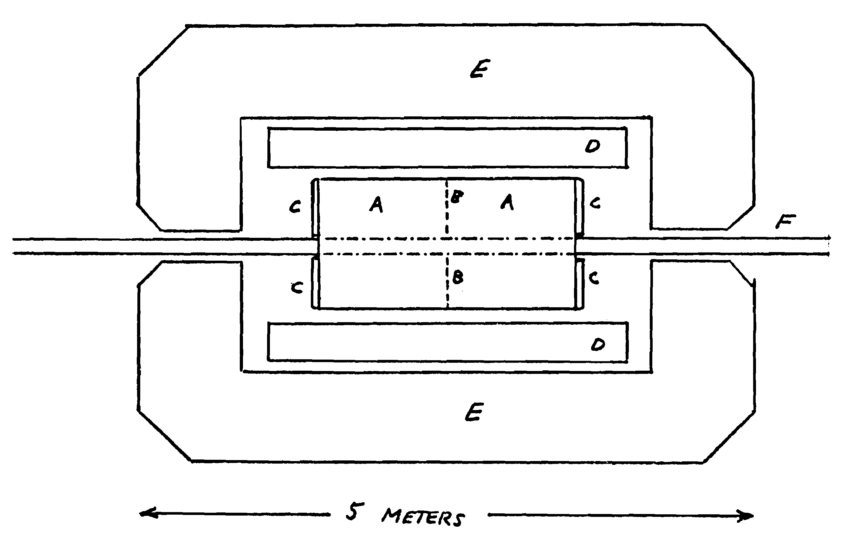
\includegraphics[width=10cm]{NygrenTPC.png}
  \caption[Original TPC design, Nygren (1974)]{The original concept of the time projection chamber particle detector, drawn by David Nygren in 1974 \cite{Nygren1974}.}
  \label{fig:NygrenTPC}
\end{figure}

The extension of this concept to a liquid argon TPC and it potential as a high-precision fine-grained detector medium in neutrino physics was proposed by Carlo Rubbia in 1977 \cite{Rubbia1977}.  The use of a noble liquid rather than gas is necessary in neutrino experiments to provide a high enough target mass to increase the probability of a neutrino interaction.  Noble liquids have high electron mobility and low diffusion, favourable properties as the detection of particles is from the ionisation and scintillation light created by the particles.  Given the necessity of a high electric field in order to drift these electrons to the readout places, excellent dielectric properties are also required; noble liquids possess such qualities.  The properties of liquid argon which make it almost perfect for this use are demonstrated in the table in Table \ref{tab:NobleProperties}.

\begin{table}
  \caption{Properties of noble elements relevant when considering a TPC medium for a neutrino experiment.}
  \label{tab:NobleProperties}
  \centering
  \begin{tabular}{ m{4cm} || m{1.3cm} | m{1.3cm} | m{1.3cm} | m{1.3cm} | m{1.3cm} | m{1.3cm} }
     & Water & He & Ne & \color{red} Ar & Kr & Xe \\
    \hline\hline
    Boiling point [K] @ 1 atm & 373 & 4.2 & 27.1 & \color{red} 87.3 & 120.0 & 165.0 \\
    \hline
    Density [g/cm$^3$] & 1 & 0.125 & 1.2 & \color{red} 1.4 & 2.4 & 3.0 \\
    \hline
    Radiation length [cm] & 36.1 & 755.2 & 24.0 & \color{red} 14.0 & 4.9 & 2.8 \\
    \hline
    Scintillation [$\gamma$/MeV] & - & 19 000 & 30 000 & \color{red} 40 000 & 25 000 & 42 000 \\
    \hline
    dE/dx [MeV/cm] & 1.9 & & 1.4 & \color{red} 2.1 & 3.0 & 3.8 \\
    \hline
    Scintillation $\lambda$ [nm] & & 80 & 78 & \color{red} 128 & 150 & 175 \\
    \hline
    Natural abundance (Earth atm) [ppm] & & 5.2 & 18.2 & \color{red} 9340.0 & 1.10 & 0.09 \\
    \hline
    Electron mobility [cm$^2$/Vs] & & low & low & \color{red} 400 & 1200 & 2200 \\
    \hline\hline
  \end{tabular}
\end{table}

An additional advantage of this technology is the low threshold for detection; this is set by the ionisation threshold of liquid argon and is only $23.6 \pm 0.5$ eV [].  Rubbia realised that a LArTPC could be the digital replacement for the high quality particle detection methods used in bubble chambers, very common in neutrino physics in the 1970s.  He proposed the first LArTPC detector design, shown in Fig. \ref{fig:RubbiaLArTPC}, which bears a striking resemblense to the LArTPC used in experiments today.

\begin{figure}
  \centering
  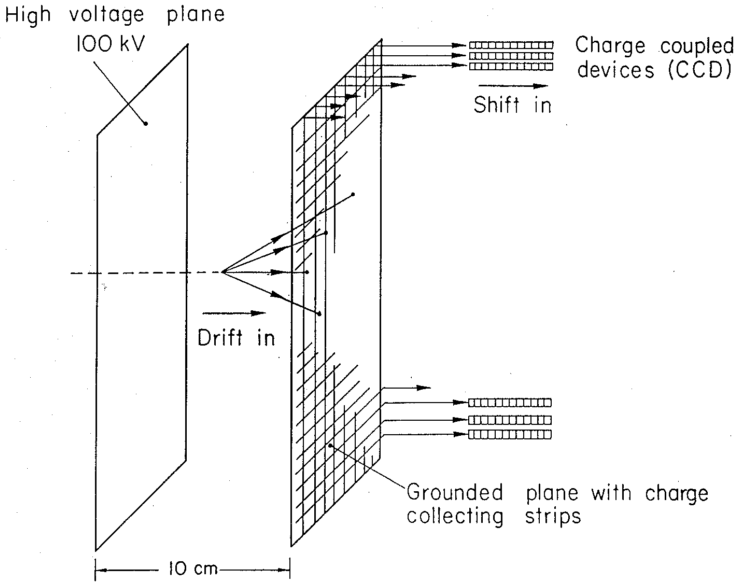
\includegraphics[width=10cm]{RubbiaLArTPC.png}
  \caption[First LArTPC detector, Rubbia (1977)]{The LArTPC detector proposed by Carlo Rubbia in 1977 \cite{Rubbia1977}.}
  \label{fig:RubbiaLArTPC}
\end{figure}

Constructing and operating such a detector was beyond the technology of the time, and is still being understood today.  The operation of a LArTPC detector and the challenges associated with this are the subject of section \ref{sec:LArTPCOperation}.

\subsection{LAr TPC Operation}\label{sec:LArTPCOperation}

explain how they work

new subsubsection

[FIND OR MAKE A FIGURE TO GO WITH THE FOLLOWING DESCRIPTION...]

A LArTPC typically consists of a single, or multiple anode and cathode, at either end of an active drift region.  An ionising particle passing through a LArTPC causes electrons to become free from argon atoms and, in the presence of a field, drift towards an anode where they are read out.

The readout consists of multiple wires planes with different orientations to facilitate the reconstruction.  The wires are either `induction' wires, which allow the electrons to deposit charge but continue past, or `collection' wires, on which the electric field lines end and all the charge on the electron is collected.  Each wire plane is therefore held at a different `bias voltage' to prevent any field lines ending on the induction wire, thus creating local electric fields which promote the continuing forward motion of the electrons.  The signal seen is therefore dependent on the type of wire plane; a bipolar pulse on an induction plane wire and unipolar on a collection plane wire.  It is also common, though not essential, to make use of a `grid plane' upstream of the signal planes in order to shield them from the electron charge until they are close.  Without such a plane, the bipolar pulse would be highly asymmetric, though would still have zero integral.  It also makes changing the drift voltage (controlling the electric field) slightly easier as the signal planes are somewhat shielded from its effects.  MicroBooNE does not operate with a grid plane and, although the 35t and the DUNE reference design make use of a grid plane, it is uncertain whether the benefit outweighs the cost for a huge LArTPC detector such as the DUNE far detector.  It is worth mentioning alternative readout possibilities have been suggested but, given the scale of future LArTPCs, it is highly unlikely a viable solution which delivers superior readout at a comparable cost will be found.


Given the positive ions that are left in the medium, there is the possibility of recombination at a later time and therefore a loss of information about the initial interaction.


This is however accompanied by a flash of scintillation light which is hugely useful as a means of determining the event `start time' ($t_0$); without this information it would be impossible to place an absolute time scale on the interaction and we would therefore not be able to resolve the coordinate along the drift direction.  The magnitude of the electric field applied is the key to both processes and there is thus a compromise which must be struck in order to preserve as much information as possible.  The graph in Fig. \ref{fig:ElectricFieldScintillationIonisation} demonstrates this; a field of $500$ V/cm is often chosen in current LAr neutrino experiments.

\begin{figure}
  \centering
  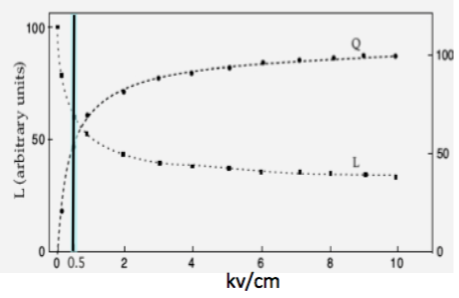
\includegraphics[width=12cm]{ElectricFieldScintillationIonisation.png}
  \caption[Affect of electric field on luminosity of ionisation electrons and scintillation light in a LArTPC]{Demonstration of the competing effect the electric field has on the luminosity of the ionisation electrons and scintillation light arriving at the detector readout.  Since both are essential in reconstructing the complete interactions, a balance must be found. [PLACEHOLDER IMAGE].}
  \label{fig:ElectronFieldScintiallationIonisation}
\end{figure}

A cathode is held at a high voltage



Flesh this stuff out...


U plane, V plane and collection all held at different fields.  Slightly increasing in order to promote forward motion of the electrons.  V held at 0V because it's cheaper (don't need crazy voltages, just some negative (still quite high, ~100V), 0V and some positive.
Grid plane (also held at potential) is to sheild the APAs from the electrons until they are close.  Not needed, but if not present then pulse wouldn't be very bipolar! The charge in both portions will still equate but the leading end will be muchhhh longer.  All electric field lines (generated from movement of electrons) end on the cathode; don't want them to end on the induction wires (hence making sure the field increases).  We want them to end on the collection planes, which collects the charge.  Signal shaping time (along with gain, the two front-end ASIC parameters) is to let the charge leave the wire before being hit again (or something like this!).  Deconvolution I still need to understand...


In 35t, we have FE ASICs which are the very front end and apply the signal shaping and gain.  Have regulators to control the power these receive (these are noisy...).  Also ADC ASICs to do digitisation in the cold.  MicroBooNE don't do this, this just have the front end and do everything else in the warm.  FE ASICs are the problem, same for uBooNE and 35t.  ADC ASIC has stuck code problem.
